\chapterimage{chapter_head_2.pdf} % Chapter heading image

%\chapter{Overview}
To manage an AGV using Robox products, 3 components are needed: a map, motion control and plant specific logic.\\

Maps are drawn using RAT software then converted to an ASCII file with \textit{.map} extension. This file is used by other two softwares: AGV manager and RDE.\\

AGV manger has two main parts: script and core. The specific logic of a plant is written in a script using XScript language, and given to the core that execute it. The core handle also the communication with the motion controller and eventually a plant PLC or database.\\

RDE is Robox IDE for motion control programming. The map is compiled by ICMap and read by the RTE. This part will be explained in other chapters.

%A block diagram of AGV is shown in fig.\ref{fig:refAgvDiag}.

\begin{figure}[h]
	\centering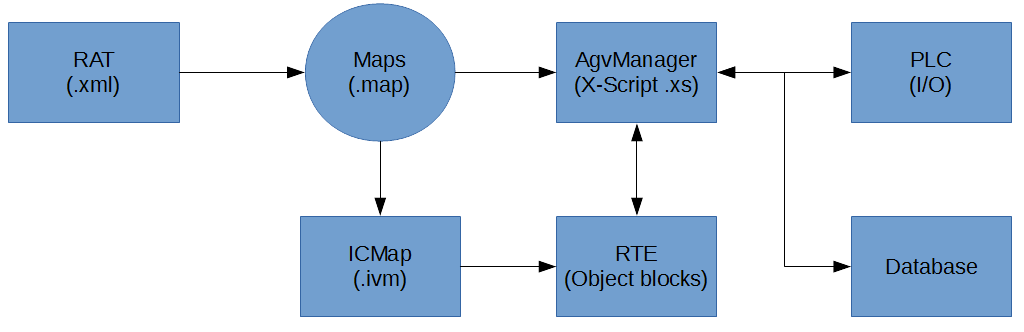
\includegraphics[scale=0.5]{agvDiag}
	\caption{AGV block diagram. RAT give a .map file as output. The map is read by AGV manager. The map is comiled by ICMap then read by RTE. AGV manager may communicate with a PLC or a database as an interface to the plant IO, and with RTE for motion control.}
	\label{fig:refAgvDiag}
\end{figure}

In the following chapters we will explain Robox software in order to draw a map and assign missions to Agv. Three softwares are needed : RAT, AgvConfigurator and AgvManager. Note that maps can also be edited by a text editor. AgvConfigurator is a part of AgvManager and are installed togethers.

